\documentclass[10pt,a4paper]{article}
\usepackage[utf8]{inputenc}
\usepackage[margin=0.6in]{geometry}
\usepackage{graphicx}
\usepackage{microtype}
\usepackage{titlesec}
\usepackage{hyperref}
\usepackage{booktabs}
\usepackage{enumitem}
\usepackage{xcolor}
\usepackage{tabularx}

\graphicspath{{certificates/}{./}}

\definecolor{amritablue}{RGB}{0, 51, 102}
\definecolor{darkgray}{RGB}{50, 50, 50}

\hypersetup{
    colorlinks=true,
    linkcolor=amritablue,
    urlcolor=amritablue,
}

\titlespacing*{\section}{0pt}{4pt}{2pt}
\titlespacing*{\subsection}{0pt}{3pt}{1pt}

\titleformat{\section}
  {\normalfont\small\bfseries\color{amritablue}\uppercase}
  {\thesection}{1em}{}[\titlerule]

\setlist{nosep, leftmargin=13pt}

\begin{document}
\pagestyle{empty}

% =========================================================
% PAGE 1: COURSE COMPLETION CERTIFICATE
% =========================================================
\begin{center}
    {\large\textbf{\color{amritablue}AMRITA VISHWA VIDYAPEETHAM}}\\[1pt]
    {\footnotesize\textbf{Amrita School of Computing, Coimbatore --- Department of Computer Science and Engineering}}\\[2pt]
    {\footnotesize\textbf{Technical Enrichment Activity: Professional Online Certification (20 Marks)}}\\[1pt]
    {\scriptsize Official Course Completion Certificate}
\end{center}

\vspace{-4pt}
\hrule height 0.8pt
\vspace{6pt}

\noindent
\begin{tabularx}{\textwidth}{@{}l X l X@{}}
    \textbf{Student Name:} & Madisetty Mounik Sai & \textbf{Course Title:} & Edge Computing Fundamentals \\
    \textbf{Roll Number:} & CB.SC.U4CSE23561 & \textbf{Platform / Provider:} & Coursera / LearnQuest \\
    \textbf{Degree \& Branch:} & B.Tech CSE (VII Semester) & \textbf{Project Guide:} & Ms. Neethu M R (Asst. Professor) \\
\end{tabularx}

\vspace{12pt}
\begin{center}
    \fbox{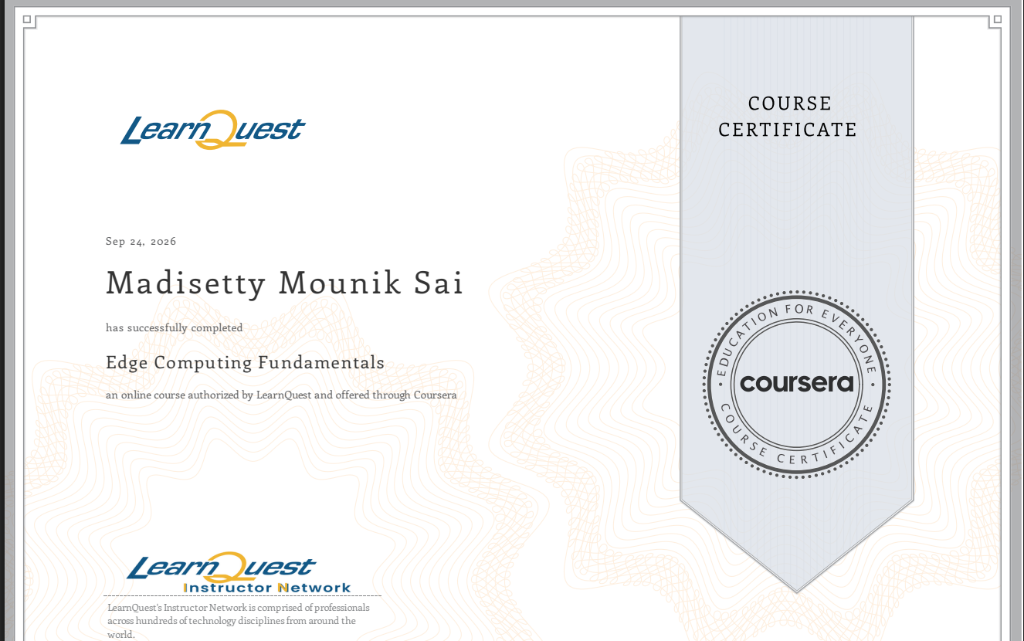
\includegraphics[width=0.96\textwidth, height=0.70\textheight, keepaspectratio]{mounik_cert.png}}
\end{center}

\vfill
\begin{center}
    {\footnotesize\textbf{Credential Verification URL:} \url{https://coursera.org/share/74f14945021f7d84329470e7e5a5361d}}
\end{center}

\clearpage

% =========================================================
% PAGE 2: TECHNICAL ALIGNMENT REPORT
% =========================================================
\begin{center}
    {\large\textbf{\color{amritablue}AMRITA VISHWA VIDYAPEETHAM}}\\[1pt]
    {\footnotesize\textbf{Amrita School of Computing, Coimbatore --- Department of Computer Science and Engineering}}\\[2pt]
    {\footnotesize\textbf{Technical Enrichment Activity: Professional Online Certification (20 Marks)}}\\[1pt]
    {\scriptsize Course Completion Details \& One-Page Technical Alignment Report}
\end{center}

\vspace{-4pt}
\hrule height 0.8pt
\vspace{4pt}

\noindent
\begin{tabularx}{\textwidth}{@{}l X l X@{}}
    \textbf{Student Name:} & Madisetty Mounik Sai & \textbf{Course Title:} & Edge Computing Fundamentals \\
    \textbf{Roll Number:} & CB.SC.U4CSE23561 & \textbf{Platform / Provider:} & Coursera / LearnQuest \\
    \textbf{Degree \& Branch:} & B.Tech CSE (VII Semester) & \textbf{Duration / Effort:} & 12--15 Hours (10--20 Hour Category) \\
    \textbf{Project Guide:} & Ms. Neethu M R (Asst. Professor) & \textbf{Verification URL:} & \url{https://coursera.org/share/74f14945021f7d84329470e7e5a5361d} \\
\end{tabularx}

\vspace{3pt}
\noindent
\textbf{B.Tech Project Title:} \textit{EdgeTrust-VANET: A Decentralized Trust Management and Machine Learning Framework for Secure Vehicular Ad Hoc Networks}

\vspace{2pt}
\section*{1. Course Curriculum \& Technical Competencies Acquired}
The professional certification \textit{Edge Computing Fundamentals} (LearnQuest via Coursera) explores the paradigms, infrastructure topologies, and data management techniques for decentralized edge computing:
\begin{itemize}
    \item \textbf{Edge vs.\ Cloud Architectural Topologies:} Evaluating round-trip latency, network jitter, bandwidth preservation, and backhaul bottleneck mitigation.
    \item \textbf{Multi-Access Edge Computing (MEC) Infrastructure:} Hierarchical tiering between local endpoints, edge gateways, fog nodes, and cloud datacenters.
    \item \textbf{Stream Data Ingestion \& Edge Aggregation:} Collecting, validating, and preprocessing high-frequency sensor telemetry at the network periphery.
    \item \textbf{Edge Reliability \& Resource Management:} Balancing edge compute capacity, power budgets, and distributed state persistence across mobile nodes.
\end{itemize}

\section*{2. Technical Justification: How the Course Directly Supports EdgeTrust-VANET}
In vehicular environments, relying on cloud infrastructure for safety verification introduces unacceptable latency ($>$24~ms), causing life-critical emergency braking advisories to arrive too late. The edge computing paradigms acquired in this course directly guided the design of our **Tier 2 Edge Roadside Unit (RSU)** and **Tier 3 Regional Fog** infrastructure:

\begin{enumerate}
    \item \textbf{Edge Infrastructure Sizing \& Latency Minimization (Tier 2 RSUs):} 
    Guided by the course's edge deployment principles, we architected Roadside Units as localized compute nodes covering an 85~m radius. Performing feature extraction and ML inference directly at the edge slashes end-to-end decision latency to \textbf{0.38~ms}---a \textbf{65$\times$ speedup} compared to traditional 24.8~ms cloud verification round-trips.

    \item \textbf{Regional Fog Computing \& Beta-Bayesian Consensus (Tier 3):} 
    The course emphasized inter-edge collaboration to prevent regional data silos. Applying this, we designed Tier 3 Regional Fog nodes connecting adjacent RSUs via low-latency local fiber rings ($<$1~ms RTT). Fog nodes execute observation-weighted Beta-Bayesian consensus with a 10-second rolling window ($W = 10$~s) to resolve boundary trust discrepancies during high-speed vehicle handovers.

    \item \textbf{Vehicular Stream Ingestion \& Feature Extraction Pipeline:} 
    Vehicles broadcast telemetry bursts at 10~Hz. Leveraging the stream ingestion techniques from the course, our edge nodes extract a 14-dimensional kinematic and reputation feature vector ($\mathbf{x} \in \mathbb{R}^{14}$) on the fly, feeding high-priority queues without dropping packets.

    \item \textbf{Multi-Source Edge Dataset Collection \& Kaggle Release:} 
    Applying edge data provenance principles, we curated our comprehensive 23,970 record benchmark across VeReMi (72.9\%), OMNeT++ (20.9\%), and V-RADD (6.3\%) edge deployments with 0.00\% cryptographic cross-split leakage, successfully open-sourcing it on Kaggle.
\end{enumerate}

\section*{3. Measurable Project Outcomes Supported by this Certification}
\noindent
\begin{tabularx}{\textwidth}{@{}X X X@{}}
    \textbf{End-to-End Latency:} 0.38~ms (65$\times$ cloud speedup) & 
    \textbf{Dataset Release:} 23,970 BSMs Published on Kaggle & 
    \textbf{Academic Status:} IEEE Conference Paper Under Review \\
\end{tabularx}

\end{document}
